\chapter{IDEMIX Based Solution}
In this chapter we will provide a solution using IDEMIX based IMS. We will give more details about how this system can be implemented, and how it will behave for the end users.
\section{IDEMIX IMS}
As in the previous cases, we can replace the IMS with \textit{IDEMIX based IMS} in our pseudonymous system as shown in figure \ref{fig:IDEMIX}. This system will take user's credentials and then send an \textit{IDEMIX token} to the bank. This IDEMIX token contains the pseudonym as well as the account ID and policy for the user. This IMS can be controlled by a separate entity inside the bank or by a 3rd party.
\begin{figure}[h]
	\centering
	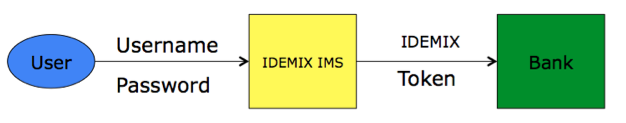
\includegraphics[width=\textwidth]{figures/IDEMIX}
	\caption{Pseudonym System with IDEMIX IMS}
	\label{fig:IDEMIX}
\end{figure}
\section{System Setup}
The system can be setup in two ways:
\begin{itemize}
	\item IMS controlled by a separate department at the bank.
	
	In this case the bank separates the authentication and service part in two different departments internally. Authentication is controlled by the IMS which holds the IDEMIX credentials for the user. The service department only gets the IDEMIX token from the authentication department.
	\item IMS controlled by a third party
	
	In this case the bank operates the service part while the authentication part is operated by a trusted third party.
\end{itemize}
In both cases, the bank and IMS have to collaborate. The bank has to trust the IMS system that the IDEMIX token sent by the the IMS system is correct.
\subsection{Changes on the Bank's Side}
In this system, the bank needs to behave as an IDEMIX \textit{issuer and verifier}. It will issue IDEMIX credentials for the users and it will also verify the tokens sent by the IMS system. 
\subsection{Information Stored at IMS}
The IMS system will behave like the user in the IDEMIX system. The IMS needs the following user information to be stored:
\begin{itemize}
	\item User IDEMIX credential
\end{itemize}
The account ID and policy can be stored in encrypted form in the credential itself. This IDEMIX credential for a particular user can be setup in the beginning and then can be used later to create authentication tokens.
\subsection{Changes needed on the User's Side}
On the user's side no changes are needed. The user accesses the system like before. He doesn't need to install any special software or hardware on his side to access the bank's services. 
\section{User Creation}
Below are the steps for the creation of a new user account in the IDEMIX based system:
\begin{itemize}
	\item The user goes to bank to open a new account.
	\item The user provides his details.
	\item The bank creates the user policy and sends this information to the IMS system along with other user information as an IDEMIX credential.
	\item The IMS system verifies the IDEMIX credential for the user and provides the user with credentials to access his account.
	\item The user can then login to his account using the credentials.
	\item In case of the corporate users, if the user is the administrator then he can add more users using a web interface at the bank directly and decide the account policies for those users.
\end{itemize}
\section{User Authentication}
Authentication steps are as following in the IDEMIX based system:
\begin{itemize}
	\item The user goes to login page.
	\item The user provides his username and password.
	\item This is sent to the IDEMIX IMS which then gets the saved user credential and creates a presentation token with a pseudonym for the bank.
	\begin{itemize}
		\item Also, for escrow purposes the real user identity is also encrypted with the public keys of authorities in the token.
	\end{itemize}
	\item The bank receives this presentation token and gets the following information:
	\begin{itemize}
		\item Pseudonym
		\item Account ID
		\item Policy
	\end{itemize}
	\item The bank adds this information in a temporary policy database.
	\item The bank saves the token for future escrow purposes.
	\item The user can then access services from the bank using the pseudonym.
	\item All user transactions are logged with the pseudonym.
\end{itemize}
\section{ID Escrow}
Following are the steps for ID escrow in the IDEMIX based system:
\begin{itemize}
	\item The authorities come to the bank for the transaction data and the IDEMIX token.
	\item After verifying, the bank gives the transaction data and corresponding IDEMIX token to the authorities.
	\item The authorities then, using their key, get the real identity of the user from the IDEMIX token.
\end{itemize}
\section{Analysis}
With the use of IDEMIX IMS we add a pseudonymous layer in the system. This provides us the necessary privacy. In order to do so, IDEMIX IMS just needs to store the IDEMIX credential of the user. 

The provider doesn’t need to store any mapping database on his side. It is easier for the  bank to implement, as the bank doesn’t really has to trust the IDEMIX IMS to store sensitive data.

In case there is a discrepancy, the authorities need to go only to the bank to get the transaction data as well as the mapping data from the IDEMIX tokens.
\section {IDEMIX implementation in the Real World}
Now we will try to fit this implementation in our system, which includes Nykredit as the Bank, Signicat as the 3rd party, DTU as the corporate customer and other government institutions as the authorities.
\subsection{Addition of the New User}
Addition of the new user can happen as follows:
\begin{enumerate}
	\item DTU registers the new user with the Nykredit giving them the user details and policies that should apply to the particular user regarding the account. 
	\begin{enumerate}
		\item Nykredit registers this new user with his user ID with the IMS system
	\end{enumerate}
	\item Nykredit issues an \textit{IDEMIX policy credential} for the given user to DTU. This credential contains the policy information and account information for the user.
	\item DTU then uses this policy credential to register the new user with Signicat. 
	\begin{enumerate}
		\item Signicat inquires about the user data with the authorities.
		\item The authorities verify the user data to Signicat.
	\end{enumerate}
	\item Signicat issues the \textit{final IDEMIX credential} for the IMS system. This credential is then used to create pseudonym IDEMIX tokens for the user. 
	The whole flow is illustrated in figure \ref{fig:IDEMIX-Real} and figure \ref{fig:Final}.
\end{enumerate}
\begin{figure}[h]
	\centering
	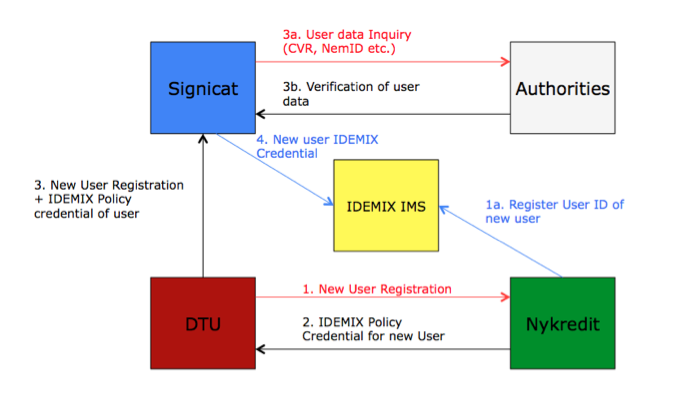
\includegraphics[width=\textwidth]{figures/IDEMIX-Real}
	\caption{IDEMIX Registration for a new user}
	\label{fig:IDEMIX-Real}
\end{figure}
\begin{figure}[h]
	\centering
	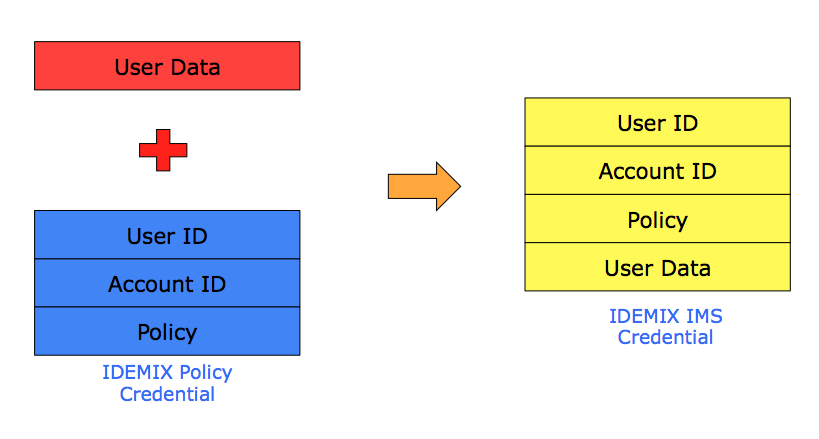
\includegraphics[width=\textwidth]{figures/Final}
	\caption{Final IDEMIX Credential from Policy Credential}
	\label{fig:Final}
\end{figure}
\FloatBarrier
\subsection{Addition of a New Customer}
Adding a new customer is almost the same as adding a new user:
\begin{enumerate}
	\item An administrator goes to Nykredit to open a bank account on behalf of DTU. 
	\begin{enumerate}
		\item Nykredit registers DTU as a new customer in their internal system.
		\item Nykredit registers the DTU administrator with his user ID with the IMS system
	\end{enumerate}
	\item Nykredit issues an IDEMIX policy credential for the DTU administrator. This credential contains the policy information and account information for the administrator.
	\item The administrator then uses his policy credential to register himslef as an owner of the new DTU account with Signicat. 
	\begin{enumerate}
		\item Signicat inquires about the data given in the credential with the authorities.
		\item The authorities verify the data to Signicat.
	\end{enumerate}
	\item Signicat issues the final IDEMIX credential for the IMS system. This credential is then used to create pseudonym IDEMIX tokens for the administrator. 
\end{enumerate}
\subsection{Technical Requirements}
In this system DTU as a client does not need to change anything on their side to be a customer at Nykredit. All the system used by DTU is web based where they can just add/remove users. Also DTU users login to the system using the normal web browser.

Nykredit has to implement \textit{IDEMIX issuer service}\cite{camenisch2002design} on their side to issue the IDEMIX Policy credential. This is done so that Nykredit doesn’t have to store the sensitive data at the 3rd party. Use of this credential ensures that this data remains safe. Nykredit also has to implement \textit{IDEMIX verifier service} to verify the user identity.

Signicat also has to implement IDEMIX issuer service to issue the final IDEMIX credential.

IMS has to implement the \textit{IDEMIX user service} to create the IDEMIX tokens for the user while the user is logging in.
\section{High Level Protocol Description}
In this section, we will give protocol description of the IDEMIX based system. This is a high level description of the protocol and full details can be found in \cite{camenisch2001efficient}.

We assume that all the systems are secured and all the communication within them is encrypted. Let $Cred_{I,U}(data1,data2,...)$ be an IDEMIX credential issued by issuer $I$ to user $U$ and $Token_{U,V}(data1,data2,...)$ be IDEMIX token created by user $U$ for verifier $V$ . We define DTU employee as entity $D$, Nykredit as entity N, IMS as entity $I$, Signicat as entity $S$ and authorities as entity $A$. Also the notation:
\begin{center}
$A \rightarrow B : \{m\}$
\end{center}
means that a message $m$ is sent from $A$ to $B$ in encrypted form such that only $A$ and $B$ can read it.
We take three cases:

\begin{enumerate}
\item User Registration
\item User Authentication
\item User transaction
\end{enumerate}
	
\subsection{User Registration}
The first part of protocol is the user registration. It involves all the parties in the system. The details of the protocol are as mentioned below:
\begin{enumerate} 
\item 	Let  $username$ be the login name of the new user that DTU wants to give access to their corporate account, $account\_id$ be the account number of DTU account with Nykredit and $policy_D$ be the policy defined by the DTU for the user on their account. DTU sends this information to the bank for the user registration.

\begin{center}
	$D \rightarrow N : \{username,account\_id,policy_D\}$
\end{center}
\begin{enumerate}
	\item The bank registers this new user with the IMS system with the given username and receives the password for the user to login to the system.
	\begin{center}
		$N \rightarrow I : \{username\}$
		
		$I \rightarrow N : \{username,password\}$
		
	\end{center}	
\end{enumerate}
\item DTU sends this password as well as an IDEMIX credential for the given username back to DTU.
	\begin{center}
		$N \rightarrow D : \{username,password,Cred_{N,D}(username,account\_id,policy_N)\}$
	\end{center}	
Where $policy_N$ is the policy created by Nykredit for the user for the given account. It is a mix of the policy given ty the DTU and also some internal Bank policies. $Cred_{N,D}(username,account\_id,policy_N)$ is the IDEMIX credential issued by Nykredit for the user with the given username.
\item DTU sends the user data and credential, given by Nykredit, to Signicat. This user data may contain \textit{real name,CPR nr,address,contact information} etc. for the user. 
\begin{center}
	$D \rightarrow S : \{username,userdata,Cred_{N,D}(username,account\_id,policy_N)\}$
\end{center}
\item Signicat verifies the user data with the authorities and then issues its own credential $Cred_{S,I}(userdata,Cred_{N,D}(account\_id,policy_N))$ for the user. This credential contains data from the Nykredit credential $Cred_{N,D}(account\_id,policy_N))$ also. This makes sure that Signicat is able to issue the credential over parameters given by Nykredit credential without need to know the data inside that credential.

Signicat sends this data to the IMS system and the user is registered with his credential in the IMS system.
\begin{center}
	$S \rightarrow I : \{username,Cred_{S,I}(userdata,Cred_{N,D}(account\_id,policy_N))\}$
\end{center}
The user can now login to the bank using the IMS system with his username and password.
\end{enumerate}

\subsection{User Authentication}
For user authentication, only DTU employee,the IMS and Nykredit systems are needed. The protocol works as follows:
\begin{enumerate}
	\item The user sends his username and password to the IMS system.
	\begin{center}
		$D \rightarrow I : \{username,password\}$
	\end{center}
	\begin{enumerate}
	\item The IMS system, after verifying the user credentials, creates an IDEMIX token from the user credential.
	\begin{center}
		$Cred_{S,I}(userdata,Cred_{N,D}(account\_id,policy_N)) \rightarrow Token_{I,N}(pseudonym,account\_id,policy_N,\{userdata\}PK_A)$
	\end{center}
	$pseudonym$ is the pseudonym generated by the IMS for the user. $Token_{I,N}(pseudonym,account\_id,policy_N,\{userdata\}PK_A)$ is the IDEMIX token created by IMS from $Cred_{S,I}(userdata,Cred_{N,D}(account\_id,policy_N))$. $PK_A$ is the public key of authorities and $userdata$ is encrypted using this public key. It is a verifiable encryption\cite{camenisch2003practical} and it can be verified that the token has actual $userdata$ encrypted using $PK_A$.
	\end{enumerate}
	\item The IMS system then sends the IDEMIX token to Nykredit. 
	\begin{center}
		$I \rightarrow N : Token_I(account\_id,policy_N,\{userdata\}PK_A)$
	\end{center}
	\item Nykredit verifies the token and authenticates the user.
	\begin{center}
		$N \rightarrow D : {pseudonym,session\_secret,status}$
	\end{center}
	Where $session\_secret$ is the secret value that Nykredit established with the user. This value is sent in subsequent requests by the user to Nykredit.
\end{enumerate}
\subsection{User Transcation}
The user transaction happens in the same manner as in the current system. We assume that the user is already authenticated using the steps above. The only entities involved are DTU user and Nykredit in this case:
\begin{enumerate}
\item The DTU user sends the transaction request to Nykredit.
	\begin{center}
		$D \rightarrow N : {session\_secret,transaction_request}$
	\end{center}
\item Nykredit performs the transcation and sends the result back.
	\begin{center}
		$N \rightarrow D : {transaction_request,status}$
	\end{center}
\end{enumerate}


This chapter described the IMS system setup using the IDEMIX system. We described how the system would be setup and how it would affect all the parties involved.


